% ============================================================================
% Introduction to Deep Equilibrium Nets (DEQNs) — Mini-Course
% March 2026
% ============================================================================

\documentclass[aspectratio=169,11pt]{beamer}

% ---------- Theme and colors ----------
\usecolortheme{dove}
\setbeamertemplate{navigation symbols}{}
\setbeamertemplate{footline}{%
  \hfill\usebeamerfont{footline}\insertframenumber\hspace*{6pt}\vskip4pt}
\setbeamerfont{footline}{size=\small}
\setbeamerfont{frametitle}{size=\huge}

% ---------- Table of contents at each section ----------
\AtBeginSection[]{%
  \begin{frame}{Outline}
    \tableofcontents[currentsection]
  \end{frame}
}
\setbeamertemplate{section in toc}[sections numbered]
\setbeamercolor{section in toc}{fg=unil@black}
\setbeamercolor{section in toc shaded}{fg=uzhgreydark}

% ---------- Packages ----------
\usepackage[utf8]{inputenc}
\usepackage[T1]{fontenc}
\usepackage{amsmath,amssymb,amsfonts}
\usepackage{bm}
\usepackage{graphicx}
\usepackage{tikz}
\usetikzlibrary{shapes,arrows.meta,positioning,calc,fit,backgrounds,patterns,decorations.pathreplacing}
\usepackage{pgfplots}
\pgfplotsset{compat=1.18}
\usepgfplotslibrary{fillbetween}
\usepackage{booktabs}
\usepackage{hyperref}
\usepackage{multicol}
\usepackage{xcolor}
\usepackage{algorithm}
\usepackage{algorithmic}
\usepackage{listings}

% ---------- Listings style for Python ----------
\lstset{
    language=Python,
    basicstyle=\small\ttfamily,
    keywordstyle=\color{uzhblue}\bfseries,
    commentstyle=\color{uzhgreydark}\itshape,
    stringstyle=\color{darkgreen},
    showstringspaces=false,
    breaklines=true,
    frame=none,
    xleftmargin=0pt,
    aboveskip=4pt,
    belowskip=4pt,
    escapeinside={(*@}{@*)},
}

% ---------- Custom colors ----------
\definecolor{uzhblue}{rgb}{0,0,0.5}
\definecolor{uzhgreylight}{RGB}{236,238,241}
\definecolor{uzhgreydark}{RGB}{81,86,94}
\definecolor{harvardcrimson}{RGB}{153,0,0}
\definecolor{unil@blue}{RGB}{0,140,204}
\definecolor{unil@black}{RGB}{35,31,32}
\definecolor{darkgreen}{RGB}{0,100,0}
\definecolor{darkred}{RGB}{139,0,0}
\definecolor{softblue}{RGB}{70,130,180}
\definecolor{softorange}{RGB}{230,159,0}
\definecolor{softgreen}{RGB}{0,158,115}

% ---------- Set beamer colors ----------
\setbeamercolor{frametitle}{bg=uzhgreylight, fg=uzhblue}
\setbeamercolor{title}{fg=uzhblue}
\setbeamercolor{structure}{fg=uzhblue}
\setbeamercolor{block title}{bg=unil@blue, fg=white}
\setbeamercolor{block body}{bg=uzhgreylight}
\setbeamercolor{block title alerted}{bg=darkred,fg=white}
\setbeamercolor{block body alerted}{bg=red!5}
\setbeamercolor{block title example}{bg=darkgreen,fg=white}
\setbeamercolor{block body example}{bg=green!5}
\setbeamercolor{item}{fg=unil@black}
\setbeamercolor{normal text}{fg=unil@black}

% ---------- Emphasis and hyperlinks ----------
\newcommand{\emphc}[1]{\textcolor{harvardcrimson}{#1}}
\hypersetup{colorlinks,linkcolor=harvardcrimson,urlcolor=harvardcrimson}

% ---------- Math commands ----------
\newcommand{\x}{\bm{x}}
\newcommand{\w}{\bm{w}}
\newcommand{\bb}{\bm{b}}
\newcommand{\z}{\bm{z}}
\newcommand{\W}{\bm{W}}
\newcommand{\X}{\bm{X}}
\renewcommand{\a}{\bm{a}}
\newcommand{\R}{\mathbb{R}}
\newcommand{\E}[1]{\mathbb{E}\!\left[#1\right]}
\DeclareMathOperator*{\argmin}{arg\,min}
\DeclareMathOperator*{\argmax}{arg\,max}

% ---------- Title ----------
\title[DEQNs --- Mini-Course]%
{Introduction to Deep Equilibrium Nets (DEQNs)}
\subtitle{A Mini-Course}
\author{Galo Nu\~{n}o \and Simon Scheidegger}
\institute[Banco de Espa\~{n}a \& HEC Lausanne]{Banco de Espa\~{n}a \and HEC, University of Lausanne}
\date{March 2026}

\begin{document}

% ============================================================================
% TITLE & OUTLINE
% ============================================================================

% --- Title ---
{\setbeamercolor{background canvas}{bg=uzhgreylight}
\begin{frame}
\titlepage
\vspace{-0.4cm}
\begin{center}
{\footnotesize Based on: Azinovic, Gaegauf \& Scheidegger (2022), \emph{International Economic Review} 63(4), 1471--1525.\\
DOI: \url{https://doi.org/10.1111/iere.12575}}\\[4pt]
{\footnotesize Materials: \url{https://github.com/sischei/DEQN_Galo_03_2026}}
\end{center}
\end{frame}
}

% --- Table of Contents ---
\begin{frame}{Course Outline}
\tableofcontents
\end{frame}


% ============================================================================
% PART I: ML/DL FOUNDATIONS
% ============================================================================

\section{ML/DL Foundations}

% --- What is ML? ---
\begin{frame}{What is Machine Learning?}
\begin{columns}[T]
\column{0.45\textwidth}
\begin{center}
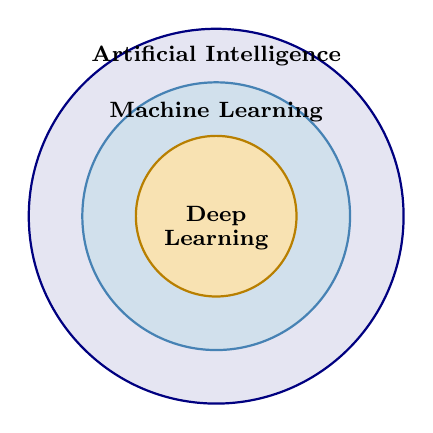
\begin{tikzpicture}[scale=0.85]
    % Concentric circles: AI > ML > DL
    \fill[uzhblue!10] (0,0) circle (2.8cm);
    \fill[softblue!25] (0,0) circle (2.0cm);
    \fill[softorange!30] (0,0) circle (1.2cm);
    \draw[uzhblue, thick] (0,0) circle (2.8cm);
    \draw[softblue, thick] (0,0) circle (2.0cm);
    \draw[softorange!80!black, thick] (0,0) circle (1.2cm);
    \node[font=\footnotesize\bfseries] at (0,0) {Deep};
    \node[font=\footnotesize\bfseries] at (0,-0.35) {Learning};
    \node[font=\footnotesize\bfseries] at (0,1.55) {Machine Learning};
    \node[font=\footnotesize\bfseries] at (0,2.4) {Artificial Intelligence};
\end{tikzpicture}
\end{center}

\column{0.52\textwidth}
\textbf{Classical programming:}

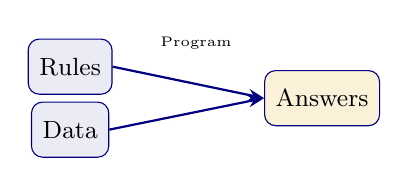
\begin{tikzpicture}[
    box/.style={rectangle, draw=uzhblue, fill=uzhblue!8, rounded corners,
                minimum height=7mm, font=\small, inner sep=4pt},
    arr/.style={-{Stealth[length=2mm]}, thick, uzhblue}]
    \node[box] (r) at (0,0) {Rules};
    \node[box] (d) at (0,-0.8) {Data};
    \node[box, fill=softorange!15] (a) at (3.2,-0.4) {Answers};
    \draw[arr] (r.east) -- (a.west);
    \draw[arr] (d.east) -- (a.west);
    \node[font=\tiny, above] at (1.6, 0.1) {Program};
\end{tikzpicture}

\vspace{0.4cm}
\textbf{Machine learning:}

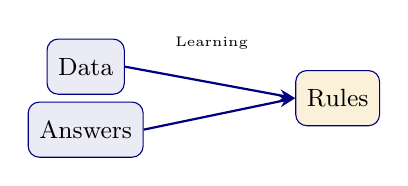
\begin{tikzpicture}[
    box/.style={rectangle, draw=uzhblue, fill=uzhblue!8, rounded corners,
                minimum height=7mm, font=\small, inner sep=4pt},
    arr/.style={-{Stealth[length=2mm]}, thick, uzhblue}]
    \node[box] (d) at (0,0) {Data};
    \node[box] (a) at (0,-0.8) {Answers};
    \node[box, fill=softorange!15] (r) at (3.2,-0.4) {Rules};
    \draw[arr] (d.east) -- (r.west);
    \draw[arr] (a.east) -- (r.west);
    \node[font=\tiny, above] at (1.6, 0.1) {Learning};
\end{tikzpicture}
\end{columns}
\end{frame}

% --- The ML Recipe ---
\begin{frame}{The Machine Learning Recipe}
Every supervised learning algorithm follows three steps:

\vspace{0.5cm}
\begin{center}
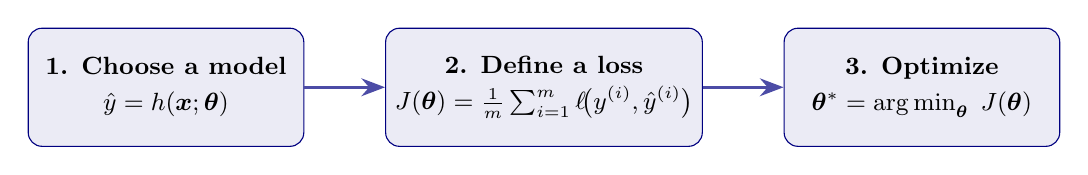
\begin{tikzpicture}[
    mlstep/.style={rectangle, draw=uzhblue, fill=uzhblue!8, rounded corners=5pt,
                 minimum width=3.5cm, minimum height=1.5cm, align=center, font=\small},
    arr/.style={-{Stealth[length=3mm]}, very thick, uzhblue!70}
]
    \node[mlstep] (m) at (0,0) {\textbf{1. Choose a model}\\[2pt]$\hat{y} = h(\x;\bm{\theta})$};
    \node[mlstep] (l) at (4.8,0) {\textbf{2. Define a loss}\\[2pt]$J(\bm{\theta}) = \frac{1}{m}\sum_{i=1}^{m}\ell\!\big(y^{(i)},\hat{y}^{(i)}\big)$};
    \node[mlstep] (o) at (9.6,0) {\textbf{3. Optimize}\\[2pt]$\bm{\theta}^{*} = \argmin_{\bm{\theta}}\; J(\bm{\theta})$};

    \draw[arr] (m) -- (l);
    \draw[arr] (l) -- (o);
\end{tikzpicture}
\end{center}

\vspace{0.5cm}
\begin{block}{Cost function example (Mean Squared Error)}
\[
    J(\bm{\theta}) \;=\; \frac{1}{2m}\sum_{i=1}^{m}\!\big(h_{\bm{\theta}}(\x^{(i)}) - y^{(i)}\big)^{2}
\]
\end{block}
\end{frame}

% --- Deep Feedforward Networks ---
\begin{frame}{Deep Feedforward Networks}
\begin{center}
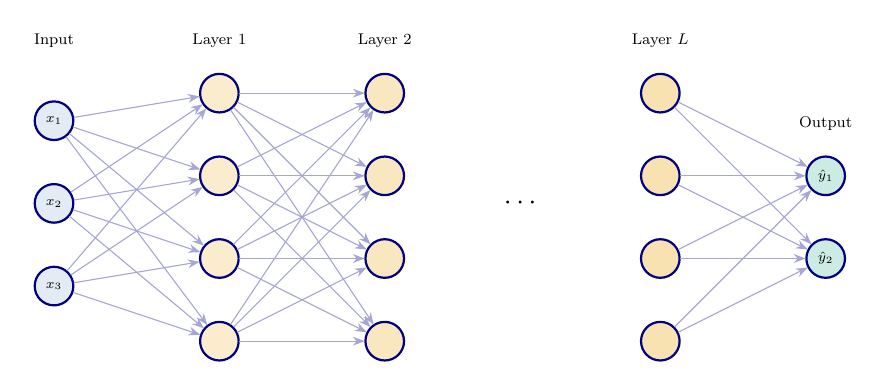
\begin{tikzpicture}[scale=0.7, transform shape,
    neuron/.style={circle, draw=uzhblue, thick, minimum size=7mm},
    arr/.style={-{Stealth[length=1.5mm]}, uzhblue!35}]

    % Input layer
    \foreach \i/\y in {1/2,2/0.5,3/-1} {
        \node[neuron, fill=softblue!15, font=\scriptsize] (x\i) at (0,\y) {$x_\i$};
    }
    % Hidden 1
    \foreach \i/\y in {1/2.5,2/1,3/-0.5,4/-2} {
        \node[neuron, fill=softorange!20, font=\tiny] (h1\i) at (3,\y) {};
    }
    % Hidden 2
    \foreach \i/\y in {1/2.5,2/1,3/-0.5,4/-2} {
        \node[neuron, fill=softorange!25, font=\tiny] (h2\i) at (6,\y) {};
    }
    % Hidden L
    \foreach \i/\y in {1/2.5,2/1,3/-0.5,4/-2} {
        \node[neuron, fill=softorange!30, font=\tiny] (hL\i) at (11,\y) {};
    }
    % Output
    \foreach \i/\y in {1/1,2/-0.5} {
        \node[neuron, fill=softgreen!20, font=\scriptsize] (y\i) at (14,\y) {$\hat{y}_\i$};
    }

    % Dots
    \node[font=\Large] at (8.5,0.5) {$\cdots$};

    % Connections
    \foreach \i in {1,2,3} { \foreach \j in {1,2,3,4} { \draw[arr] (x\i)--(h1\j); }}
    \foreach \i in {1,2,3,4} { \foreach \j in {1,2,3,4} { \draw[arr] (h1\i)--(h2\j); }}
    \foreach \i in {1,2,3,4} { \foreach \j in {1,2} { \draw[arr] (hL\i)--(y\j); }}

    % Layer labels
    \node[font=\footnotesize, above] at (0,3.2) {Input};
    \node[font=\footnotesize, above] at (3,3.2) {Layer 1};
    \node[font=\footnotesize, above] at (6,3.2) {Layer 2};
    \node[font=\footnotesize, above] at (11,3.2) {Layer $L$};
    \node[font=\footnotesize, above] at (14,1.7) {Output};
\end{tikzpicture}
\end{center}

\vspace{0.1cm}
An $L$-layer network computes a nested composition:
\[
    \boxed{f(\x;\bm{\theta}) = g_L\!\Big(\W^{(L)} g_{L-1}\!\big(\cdots g_1\!\big(\W^{(1)}\x + \bb^{(1)}\big)\cdots + \bb^{(L-1)}\big) + \bb^{(L)}\Big)}
\]

{\small Each layer transforms the representation.  \textbf{Depth} provides exponential gains in representational power over width alone.}
\end{frame}

% --- Universal Approximation ---
\begin{frame}{Universal Approximation Theorem}
\begin{block}{Theorem (Cybenko 1989; Hornik, Stinchcombe \& White 1989)}
{\small Let $g:\R\to\R$ be a bounded, non-constant, continuous activation function.  Then for any continuous function $f:\mathcal{K}\to\R$ on a compact set $\mathcal{K}\subset\R^d$ and any $\varepsilon>0$, there exists a single-hidden-layer network
\vspace{-0.2cm}
\[
    F(\x) = \sum_{j=1}^{n_1} v_j\, g\!\big(\w_j^\top\x + b_j\big)
\]
\vspace{-0.4cm}

such that $\sup_{\x\in\mathcal{K}} |F(\x) - f(\x)| < \varepsilon$.}
\end{block}

\vspace{0.1cm}
{\small\textbf{Caveats:}
\begin{itemize}\itemsep1pt
    \item The required width $n_1$ may be \textbf{exponentially large} in $d$.
    \item Existence $\neq$ efficient learnability.
    \item Practical success of deep learning suggests that \textbf{depth} provides a much more efficient parameterization than width alone.
\end{itemize}}
\end{frame}

% --- Activation Functions ---
\begin{frame}{Activation Functions}
\begin{center}
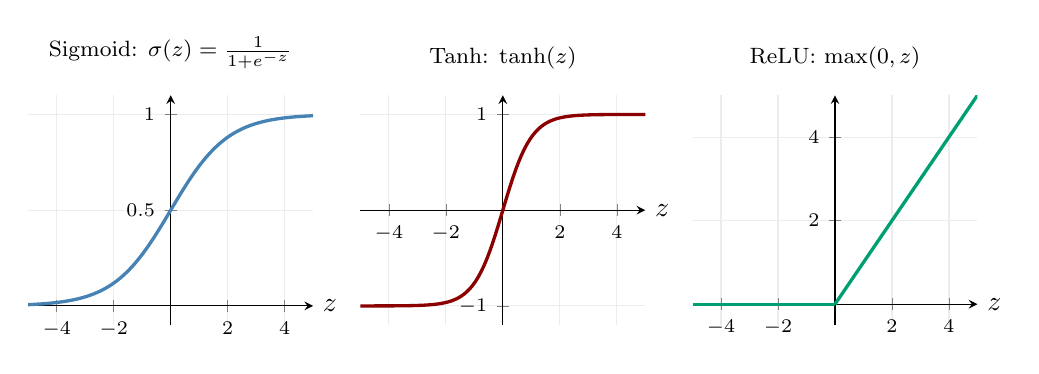
\begin{tikzpicture}
\begin{axis}[
    name=plot1,
    width=5.2cm, height=4.5cm,
    title={\footnotesize Sigmoid: $\sigma(z) = \frac{1}{1+e^{-z}}$},
    title style={font=\footnotesize},
    xlabel={$z$}, xlabel style={font=\scriptsize},
    tick label style={font=\scriptsize},
    xmin=-5, xmax=5, ymin=-0.1, ymax=1.1,
    grid=major, grid style={gray!15},
    axis lines=middle,
    every axis x label/.style={at={(current axis.right of origin)}, anchor=west},
]
    \addplot[very thick, softblue, domain=-5:5, samples=100]{1/(1+exp(-x))};
\end{axis}

\begin{axis}[
    at={($(plot1.east)+(0.6cm,0)$)}, anchor=west,
    name=plot2,
    width=5.2cm, height=4.5cm,
    title={\footnotesize Tanh: $\tanh(z)$},
    title style={font=\footnotesize},
    xlabel={$z$}, xlabel style={font=\scriptsize},
    tick label style={font=\scriptsize},
    xmin=-5, xmax=5, ymin=-1.2, ymax=1.2,
    grid=major, grid style={gray!15},
    axis lines=middle,
    every axis x label/.style={at={(current axis.right of origin)}, anchor=west},
]
    \addplot[very thick, darkred, domain=-5:5, samples=100]{tanh(x)};
\end{axis}

\begin{axis}[
    at={($(plot2.east)+(0.6cm,0)$)}, anchor=west,
    name=plot3,
    width=5.2cm, height=4.5cm,
    title={\footnotesize ReLU: $\max(0,z)$},
    title style={font=\footnotesize},
    xlabel={$z$}, xlabel style={font=\scriptsize},
    tick label style={font=\scriptsize},
    xmin=-5, xmax=5, ymin=-0.5, ymax=5,
    grid=major, grid style={gray!15},
    axis lines=middle,
    every axis x label/.style={at={(current axis.right of origin)}, anchor=west},
]
    \addplot[very thick, softgreen, domain=-5:0, samples=2]{0};
    \addplot[very thick, softgreen, domain=0:5, samples=2]{x};
\end{axis}
\end{tikzpicture}
\end{center}

\vspace{0.2cm}
{\small Other common activations: \emphc{Leaky ReLU} $\max(0.01z, z)$, \emphc{Softplus} $\ln(1+e^z)$, \emphc{ELU}, \emphc{Swish} $z\cdot\sigma(z)$.}
\end{frame}

% --- DNN Layer Structure ---
\begin{frame}{DNN Layer Structure}
\begin{center}
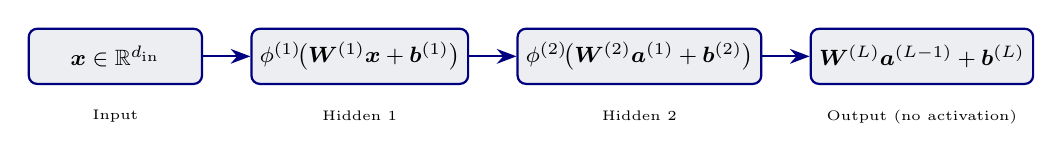
\begin{tikzpicture}[
    mlstep/.style={rectangle, draw=uzhblue, thick, fill=uzhgreylight,
        minimum width=2.2cm, minimum height=0.7cm, font=\footnotesize,
        rounded corners=3pt, inner sep=3pt},
    arr/.style={-{Stealth[length=2.5mm]}, thick, uzhblue}
]
    \node[mlstep] (in) {$\x \in \R^{d_{\text{in}}}$};
    \node[mlstep, right=0.6cm of in] (h1) {$\phi^{(1)}\!\bigl(\W^{(1)}\x + \bb^{(1)}\bigr)$};
    \node[mlstep, right=0.6cm of h1] (h2) {$\phi^{(2)}\!\bigl(\W^{(2)}\a^{(1)} + \bb^{(2)}\bigr)$};
    \node[mlstep, right=0.6cm of h2] (out) {$\W^{(L)}\a^{(L-1)} + \bb^{(L)}$};

    \draw[arr] (in) -- (h1);
    \draw[arr] (h1) -- (h2);
    \draw[arr] (h2) -- (out);

    \node[below=0.2cm, font=\tiny] at (in.south) {Input};
    \node[below=0.2cm, font=\tiny] at (h1.south) {Hidden 1};
    \node[below=0.2cm, font=\tiny] at (h2.south) {Hidden 2};
    \node[below=0.2cm, font=\tiny] at (out.south) {Output (no activation)};
\end{tikzpicture}
\end{center}

\vspace{0.3em}
Each hidden layer applies a \emphc{nonlinear activation} $\phi^{(\ell)}$:
\[
\a^{(\ell)} = \phi^{(\ell)}\!\bigl(\W^{(\ell)} \a^{(\ell-1)} + \bb^{(\ell)}\bigr), \qquad \ell = 1, \ldots, L-1
\]

\vspace{0.2em}
\begin{itemize}
    \item The output layer is typically \emphc{linear} (for regression) or uses \emphc{softplus} (to enforce positivity, e.g.\ consumption)
    \item The full network: $\mathcal{N}_\rho(\x) = \W^{(L)} \a^{(L-1)} + \bb^{(L)}$
\end{itemize}
\end{frame}

% --- Gradient Descent ---
\begin{frame}{Gradient Descent and SGD}
\begin{columns}[T]
\column{0.48\textwidth}
\textbf{Goal:} find weights that minimize the loss:
\[
    \bm{\theta}^{*} = \argmin_{\bm{\theta}}\; J(\bm{\theta})
\]

\textbf{Strategy:} repeatedly step in the direction of steepest descent:
\[
    \bm{\theta} \;\leftarrow\; \bm{\theta} - \eta\,\nabla_{\!\bm{\theta}} J(\bm{\theta})
\]

\vspace{0.3em}
\textbf{Mini-batch SGD:} sample a batch $\mathcal{B}$ of $B$ examples:
\[
    \bm{\theta} \leftarrow \bm{\theta} - \frac{\eta}{B}\sum_{k\in\mathcal{B}} \nabla_{\!\bm{\theta}} J_k(\bm{\theta})
\]

\column{0.48\textwidth}
\begin{center}
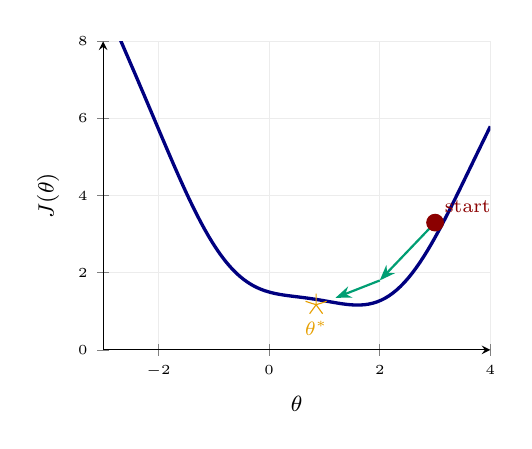
\begin{tikzpicture}
\begin{axis}[
    width=6.5cm, height=5.5cm,
    xlabel={$\theta$}, ylabel={$J(\theta)$},
    xlabel style={font=\footnotesize},
    ylabel style={font=\footnotesize},
    tick label style={font=\tiny},
    xmin=-3, xmax=4, ymin=0, ymax=8,
    grid=major, grid style={gray!15},
    axis lines=left,
    ytick={0,2,4,6,8},
]
    % Loss curve
    \addplot[very thick, uzhblue, domain=-3:4, samples=100]{0.5*(x-1)^2 + 0.3*sin(deg(x*2)) + 1};
    % Starting point
    \addplot[only marks, mark=*, mark size=3pt, darkred] coordinates {(3, 3.3)};
    \node[font=\scriptsize, darkred, above right] at (axis cs:3,3.3) {start};
    % Arrow showing descent
    \draw[-{Stealth[length=2mm]}, thick, softgreen] (axis cs:3,3.3) -- (axis cs:2,1.8);
    \draw[-{Stealth[length=2mm]}, thick, softgreen] (axis cs:2,1.8) -- (axis cs:1.2,1.35);
    % Minimum
    \addplot[only marks, mark=star, mark size=4pt, softorange] coordinates {(0.85, 1.17)};
    \node[font=\scriptsize, softorange, below] at (axis cs:0.85,1.0) {$\theta^*$};
\end{axis}
\end{tikzpicture}
\end{center}
\end{columns}
\end{frame}

% --- Loss Functions ---
\begin{frame}{Loss Functions}
The loss function $J(\bm{\theta})$ measures how far predictions $\hat{\bm{y}}$ are from targets $\bm{y}$.

\vspace{0.4cm}
\begin{columns}[T]
\column{0.48\textwidth}
\begin{block}{Regression: Mean Squared Error}
\[
    J(\bm{\theta}) = \frac{1}{2n}\sum_{i=1}^{n}\big(y^{(i)} - f(\x^{(i)};\bm{\theta})\big)^{2}
\]
Penalizes large deviations quadratically.
\end{block}

\column{0.48\textwidth}
\begin{block}{Classification: Cross-Entropy}
{\small
\[
    J = -\frac{1}{n}\sum_{i=1}^{n}\!\Big[y^{(i)}\!\log\hat{y}^{(i)} + (1{-}y^{(i)})\log(1{-}\hat{y}^{(i)})\Big]
\]}%
\vspace{-0.3cm}

For binary labels $y\in\{0,1\}$.
\end{block}
\end{columns}

\vspace{0.3cm}
{\small In computational economics, we will replace labeled data with \emphc{structural equations}---the key insight behind DEQNs.}
\end{frame}

% --- Why Deep Learning Now? ---
\begin{frame}{Why Deep Learning Now?}
Neural networks date back to the 1940s.  Three developments made them practical:

\vspace{0.4cm}
\begin{center}
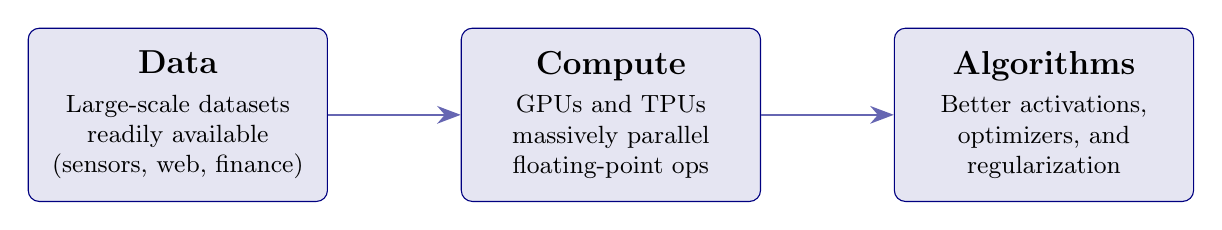
\begin{tikzpicture}[
    box/.style={rectangle, draw=uzhblue, fill=uzhblue!10, rounded corners=4pt,
                minimum width=3.8cm, minimum height=2.2cm, align=center, font=\small},
    arr/.style={-{Stealth[length=3mm]}, thick, uzhblue!60}
]
    \node[box] (data) at (0,0) {\textbf{\large Data}\\[3pt]Large-scale datasets\\readily available\\(sensors, web, finance)};
    \node[box] (hw) at (5.5,0) {\textbf{\large Compute}\\[3pt]GPUs and TPUs\\massively parallel\\floating-point ops};
    \node[box] (sw) at (11,0) {\textbf{\large Algorithms}\\[3pt]Better activations,\\optimizers, and\\regularization};

    \draw[arr] (data) -- (hw);
    \draw[arr] (hw) -- (sw);
\end{tikzpicture}
\end{center}

\vspace{0.3cm}
{\small Key milestones: Perceptron (1958), Backpropagation (1986), Deep CNN (1995), AlexNet (2012), Transformers (2017), ChatGPT (2022).}
\end{frame}


% ============================================================================
% PART II: DEEP EQUILIBRIUM NETS
% ============================================================================

\section{Deep Equilibrium Nets}

% --- Heterogeneity Matters ---
\begin{frame}{Heterogeneity Matters}
\begin{columns}[T]
\column{0.48\textwidth}
\textbf{Key questions in macroeconomics:}
\begin{itemize}
    \item How does \emphc{inequality} evolve over the life cycle?
    \item How do \emphc{idiosyncratic shocks} interact with aggregate risk?
    \item What are the \emphc{distributional effects} of policy?
\end{itemize}

\vspace{0.5em}
$\Rightarrow$ Need \emphc{overlapping-generations} (OLG) models with many heterogeneous agents.

\column{0.48\textwidth}
\begin{center}
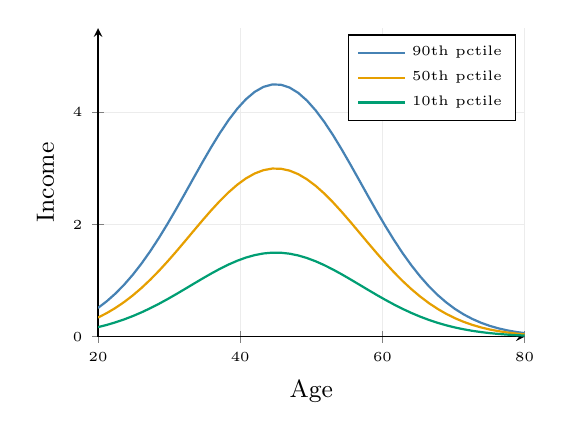
\begin{tikzpicture}
\begin{axis}[
    width=7cm, height=5.5cm,
    xlabel={Age}, ylabel={Income},
    xlabel style={font=\small},
    ylabel style={font=\small},
    tick label style={font=\tiny},
    xmin=20, xmax=80, ymin=0, ymax=5.5,
    grid=major, grid style={gray!15},
    legend style={font=\tiny, at={(0.98,0.98)}, anchor=north east},
    axis lines=left,
]
    \addplot[thick, softblue, domain=20:80, samples=50]
        {4.5*exp(-0.5*((x-45)/12)^2)};
    \addlegendentry{90th pctile}
    \addplot[thick, softorange, domain=20:80, samples=50]
        {3.0*exp(-0.5*((x-45)/12)^2)};
    \addlegendentry{50th pctile}
    \addplot[thick, softgreen, domain=20:80, samples=50]
        {1.5*exp(-0.5*((x-45)/12)^2)};
    \addlegendentry{10th pctile}
\end{axis}
\end{tikzpicture}\\
{\tiny Stylized income-by-age profiles}
\end{center}
\end{columns}
\end{frame}

% --- DSGE Models ---
\begin{frame}{Dynamic Stochastic General Equilibrium Models}
\textbf{Generic formulation:} find policy functions $p(\cdot)$ such that
\[
\E{G\bigl(\x_t,\,\x_{t+1},\,p(\x_t),\,p(\x_{t+1})\bigr) \;\Big|\; \x_t,\,p(\x_t)} = 0
\]
with transition law $\x_{t+1} = h\bigl(\x_t,\,p(\x_t),\,\varepsilon_{t+1}\bigr)$.

\vspace{0.6em}
\textbf{Challenges:}
\begin{itemize}
    \item State space $\x_t \in \R^d$ can be \emphc{very high-dimensional}
    \item Standard grid-based methods scale as $\mathcal{O}(n^d)$~~$\Rightarrow$~~\emphc{curse of dimensionality}
    \item Need a method that \emphc{does not rely on grids}
\end{itemize}
\end{frame}

% --- What is High-Dimensional? ---
\begin{frame}{What is High-Dimensional?}
\begin{center}
\begin{tabular}{rrl}
\toprule
\textbf{Dimensions $d$} & \textbf{Grid points $n^d$} & \textbf{Runtime} \\
\midrule
1 & $10$ & 10 seconds \\
2 & $100$ & 2 minutes \\
5 & $10^5$ & 1 day \\
10 & $10^{10}$ & 317 years \\
20 & $10^{20}$ & $\sim 3$ trillion years \\
\bottomrule
\end{tabular}
\end{center}

\vspace{0.5em}
{\small Assumes $n = 10$ grid points per dimension and 1 second per evaluation.}

\vspace{0.5em}
\textbf{Three remedies:}
\begin{enumerate}
    \item \emphc{Sparse grids}~(Brumm \& Scheidegger, 2017)
    \item \emphc{Random grids}~(Rust, 1997)
    \item \emphc{Neural networks}~(this lecture)
\end{enumerate}
\end{frame}

% --- Volumes in High Dimensions ---
\begin{frame}{Volumes in High Dimensions}
\begin{center}
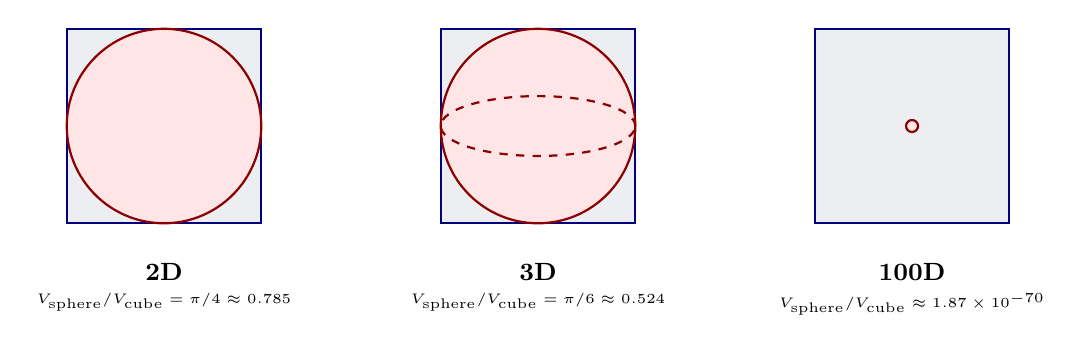
\begin{tikzpicture}[scale=0.95]
% 2D
\begin{scope}[shift={(0,0)}]
    \draw[thick, uzhblue, fill=uzhgreylight] (-1.3,-1.3) rectangle (1.3,1.3);
    \draw[thick, darkred, fill=red!10] (0,0) circle (1.3);
    \node[below, font=\small\bfseries] at (0,-1.7) {2D};
    \node[below, font=\tiny] at (0,-2.1) {$V_{\text{sphere}}/V_{\text{cube}} = \pi/4 \approx 0.785$};
\end{scope}
% 3D
\begin{scope}[shift={(5,0)}]
    \draw[thick, uzhblue, fill=uzhgreylight] (-1.3,-1.3) rectangle (1.3,1.3);
    \draw[thick, darkred, fill=red!10] (0,0) circle (1.3);
    \draw[thick, darkred, dashed] (0,0) ellipse (1.3 and 0.4);
    \node[below, font=\small\bfseries] at (0,-1.7) {3D};
    \node[below, font=\tiny] at (0,-2.1) {$V_{\text{sphere}}/V_{\text{cube}} = \pi/6 \approx 0.524$};
\end{scope}
% 100D
\begin{scope}[shift={(10,0)}]
    \draw[thick, uzhblue, fill=uzhgreylight] (-1.3,-1.3) rectangle (1.3,1.3);
    \draw[thick, darkred, fill=red!10] (0,0) circle (0.08);
    \node[below, font=\small\bfseries] at (0,-1.7) {100D};
    \node[below, font=\tiny] at (0,-2.1) {$V_{\text{sphere}}/V_{\text{cube}} \approx 1.87 \times 10^{-70}$};
\end{scope}
\end{tikzpicture}
\end{center}

\vspace{0.4em}
\begin{block}{Implication}
In high dimensions, \emphc{almost all volume is in the corners}. Grid-based methods waste most of their evaluation points in regions that barely contribute to the integral or approximation.
\end{block}
\end{frame}

% --- Our Solution: DEQNs ---
\begin{frame}{Our Solution: Deep Equilibrium Nets}
\textbf{Core idea} (Azinovic, Gaegauf \& Scheidegger, 2022):

\vspace{0.3em}
Replace the traditional grid-based solution with a \emphc{neural network} trained to satisfy economic equilibrium conditions.

\vspace{0.5em}
\begin{block}{Three Key Ingredients}
\begin{enumerate}
    \item \textbf{Equilibrium error as loss function:} use the economic equations $G(\cdot) = 0$ directly---\emphc{no labeled data} needed
    \item \textbf{Stochastic gradient descent:} optimize network parameters $\rho$ via SGD on mini-batches
    \item \textbf{Simulated paths:} draw training points from the \emphc{ergodic distribution} of the model itself
\end{enumerate}
\end{block}

\vspace{0.3em}
{\small $\Rightarrow$ This turns \emphc{solving} an economic model into \emphc{training} a neural network.}
\end{frame}

% --- What is a DNN? ---
\begin{frame}{What is a Deep Neural Network?}
A deep neural network (DNN) $\mathcal{N}_\rho : \R^{d_{\text{in}}} \to \R^{d_{\text{out}}}$ is a \emphc{parametric function approximator}.

\vspace{0.5em}
\textbf{Universal approximation} (Cybenko 1989, Hornik 1991):
\[
\text{For any continuous } f : \mathcal{K} \to \R \text{ and } \varepsilon > 0, \;\; \exists\, \rho^\star : \quad \|\mathcal{N}_{\rho^\star} - f\| < \varepsilon
\]

\vspace{0.5em}
\textbf{In economics:}
\begin{itemize}
    \item \emphc{Input:} state variables $\x_t \in \R^{d}$ (capital, productivity, wealth distribution, \ldots)
    \item \emphc{Output:} policy variables (consumption, savings, prices, \ldots)
    \item \emphc{Parameters} $\rho$: weights and biases---found by \emphc{training}
\end{itemize}
\end{frame}

% --- The Data Problem ---
\begin{frame}{The ``Data Problem'' in Economics}
\textbf{Deep learning excels} when massive labeled datasets are available.

\vspace{0.5em}
\textbf{But in computational economics:}
\begin{itemize}
    \item We solve \emphc{functional equations}, not classification/regression tasks
    \item There are \emphc{no labeled pairs} $(\x_i, y_i)$
    \item Traditional approach: \emphc{time iteration on a grid}---but grids do not scale
\end{itemize}

\vspace{0.5em}
\textbf{Key insight:}
\begin{itemize}
    \item We \emphc{know} the structural equations $G(\cdot) = 0$
    \item We can \emphc{check} how well a candidate policy satisfies them
    \item $\Rightarrow$ Use the \emphc{equilibrium error} as the loss function!
\end{itemize}
\end{frame}

% --- Traditional Approach ---
\begin{frame}{Traditional Approach: Time Iteration on a Grid}
\begin{alertblock}{Algorithm: Grid-Based Collocation}
\begin{algorithmic}
\small
\STATE \textbf{Input:} Grid $\mathcal{G} = \{\x_1, \ldots, \x_M\} \subset \R^d$, initial guess $p^{(0)}$
\FOR{$k = 0, 1, 2, \ldots$ until convergence}
    \FOR{each grid point $\x_i \in \mathcal{G}$}
        \STATE Solve $G\bigl(\x_i,\, p^{(k)}(\x_i),\, p^{(k)}\bigr) = 0$ for $p^{(k+1)}(\x_i)$
    \ENDFOR
    \STATE Interpolate $p^{(k+1)}$ between grid points
\ENDFOR
\end{algorithmic}
\end{alertblock}

\vspace{0.3em}
\textbf{Problems:}
\begin{itemize}
    \item Grid size $M = n^d$ $\Rightarrow$ \emphc{exponential} in dimension $d$
    \item Interpolation in $d > 5$ becomes expensive and inaccurate
    \item Cannot handle models with $d = 60$ or more state variables
\end{itemize}
\end{frame}

% --- DEQN Loss Function ---
\begin{frame}{The DEQN Loss Function}
\textbf{Key idea:} replace labeled data with \emphc{economic equilibrium conditions}.

\vspace{0.5em}
Let $G(\x, f(\x)) = 0$ be the system of equilibrium equations. Define:
\[
\boxed{
\ell_\rho = \frac{1}{N} \sum_{i=1}^{N} \bigl\| G\bigl(\x_i,\, \mathcal{N}_\rho(\x_i)\bigr) \bigr\|^2
}
\]

\vspace{0.3em}
\begin{itemize}
    \item $\mathcal{N}_\rho(\x_i)$ is the neural net's \emphc{predicted policy} at state $\x_i$
    \item $G(\cdot)$ measures the \emphc{equilibrium error} (e.g.\ Euler equation residual)
    \item $\ell_\rho = 0$ iff the policy \emphc{exactly} satisfies all equilibrium conditions
\end{itemize}

\vspace{0.5em}
$\Rightarrow$ \emphc{No labels needed}---this is \textbf{unsupervised} (or ``self-supervised'') learning.
\end{frame}

% --- DEQN Training Algorithm ---
\begin{frame}{Training Algorithm for DEQNs}
\begin{block}{Algorithm 1: Deep Equilibrium Net Training}
\begin{algorithmic}
\footnotesize
\STATE \textbf{Input:} Initial state $\x_0$, network $\mathcal{N}_\rho$, learning rate $\alpha$, \# episodes $E$, \# epochs $T$
\FOR{episode $e = 1, \ldots, E$}
    \STATE \textbf{Simulate path:} $\x_0 \to \x_1 \to \cdots \to \x_T$ using $\mathcal{N}_\rho$ and transition law
    \FOR{epoch $t = 1, \ldots, T$}
        \STATE Draw mini-batch $\mathcal{B} \subset \{\x_0, \ldots, \x_T\}$
        \STATE Compute loss:~$\ell_\rho = \frac{1}{|\mathcal{B}|}\sum_{\x_i \in \mathcal{B}} \|G(\x_i, \mathcal{N}_\rho(\x_i))\|^2$
        \STATE Update:~$\rho \leftarrow \rho - \alpha \cdot \nabla_\rho \ell_\rho$
    \ENDFOR
\ENDFOR
\STATE \textbf{Output:} Trained network $\mathcal{N}_{\rho^\star}$ approximating the policy function
\end{algorithmic}
\end{block}

\vspace{0.2em}
{\small \textbf{Note:} Training points come from the \emphc{model's own simulation}---the network learns on the ergodic distribution, focusing on economically relevant regions.}
\end{frame}

% --- Supervised vs Unsupervised ---
\begin{frame}{Supervised vs.\ Unsupervised (DEQN) Learning}
\begin{columns}[T]
\column{0.47\textwidth}
\begin{center}
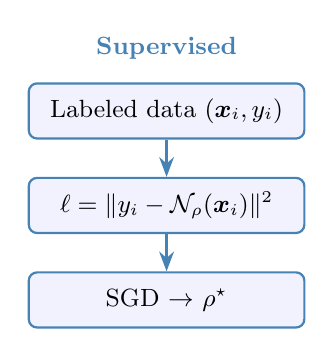
\begin{tikzpicture}[
    mlstep/.style={rectangle, draw=softblue, thick, fill=blue!5,
        minimum width=3.5cm, minimum height=0.7cm, font=\small,
        rounded corners=3pt},
    arr/.style={-{Stealth[length=2.5mm]}, thick, softblue}
]
    \node[font=\small\bfseries, softblue] at (0,3.2) {Supervised};
    \node[mlstep] (d) at (0,2.4) {Labeled data $(\x_i, y_i)$};
    \node[mlstep] (l) at (0,1.2) {$\ell = \|y_i - \mathcal{N}_\rho(\x_i)\|^2$};
    \node[mlstep] (s) at (0,0) {SGD $\to$ $\rho^\star$};
    \draw[arr] (d) -- (l);
    \draw[arr] (l) -- (s);
\end{tikzpicture}
\end{center}

\column{0.47\textwidth}
\begin{center}
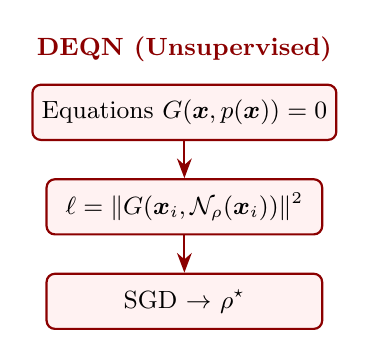
\begin{tikzpicture}[
    mlstep/.style={rectangle, draw=darkred, thick, fill=red!5,
        minimum width=3.5cm, minimum height=0.7cm, font=\small,
        rounded corners=3pt},
    arr/.style={-{Stealth[length=2.5mm]}, thick, darkred}
]
    \node[font=\small\bfseries, darkred] at (0,3.2) {DEQN (Unsupervised)};
    \node[mlstep] (d) at (0,2.4) {Equations $G(\x, p(\x))=0$};
    \node[mlstep] (l) at (0,1.2) {$\ell = \|G(\x_i, \mathcal{N}_\rho(\x_i))\|^2$};
    \node[mlstep] (s) at (0,0) {SGD $\to$ $\rho^\star$};
    \draw[arr] (d) -- (l);
    \draw[arr] (l) -- (s);
\end{tikzpicture}
\end{center}
\end{columns}

\vspace{0.5em}
\begin{center}
{\small \emphc{Key difference:} DEQNs replace labeled data with structural economic equations.}
\end{center}
\end{frame}

% --- The Cost of Labeled Data ---
\begin{frame}{The Cost of Labeled Data in Economics}
\textbf{Supervised learning requires labeled pairs $(\x_i, y_i)$.}

\vspace{0.3em}
In computational economics, generating a single label $y_i$ means \emphc{solving the model} at state $\x_i$---precisely the problem we are trying to solve!

\vspace{0.4em}
\begin{center}
\renewcommand{\arraystretch}{1.35}
{\small
\begin{tabular}{@{}lll@{}}
\toprule
\textbf{Step} & \textbf{Supervised (label generation)} & \textbf{DEQN (unsupervised)} \\
\midrule
1 & Choose grid $\mathcal{G}$ of $n^d$ points & Draw states from simulation \\
2 & \emphc{Solve} $G(\x_i, y_i) = 0$ at each $\x_i$ & Evaluate residual $G(\x_i, \mathcal{N}_\rho(\x_i))$ \\
3 & Fit $\hat{y} = f(\x; \bm{\theta})$ to $\{(\x_i, y_i)\}$ & Update $\rho$ via SGD on residual \\
\midrule
Cost & $\underbrace{n^d}_{\text{grid}} \times \underbrace{C_{\text{solve}}}_{\text{per point}}$ + fitting & $E \times T \times \underbrace{B}_{\text{batch}} \times C_{\text{residual}}$ \\
\bottomrule
\end{tabular}
}
\end{center}

\vspace{0.4em}
{\small
\begin{itemize}
    \item $C_{\text{solve}}$: cost of solving a nonlinear system or iterating a Bellman equation to convergence
    \item $C_{\text{residual}}$: cost of a single forward pass through the equilibrium equations---\emphc{orders of magnitude cheaper}
\end{itemize}
}
\end{frame}

% --- Why Supervised Learning is Expensive ---
\begin{frame}{Why Supervised Learning is Prohibitively Expensive}
\textbf{To generate labels}, we must solve the model on a grid. This involves:

\vspace{0.3em}
\begin{columns}[T]
\column{0.48\textwidth}
\begin{alertblock}{1. Bellman / value function iteration}
\begin{itemize}
    \item Iterate $V_{k+1}(\x) = \max_a \{u(a) + \beta \E{V_k(\x')}\}$
    \item Each iteration: solve $n^d$ optimisation problems
    \item Typically $\mathcal{O}(100)$ iterations to converge
    \item Interpolation between grid points introduces error
\end{itemize}
\end{alertblock}

\column{0.48\textwidth}
\begin{alertblock}{2. Nonlinear system solving}
\begin{itemize}
    \item At each $\x_i$: solve $G(\x_i, y) = 0$ via Newton's method
    \item Each Newton step: compute and invert a Jacobian
    \item Cost per point: $\mathcal{O}(m^3)$ for $m$ equations
    \item Convergence not guaranteed away from the solution
\end{itemize}
\end{alertblock}
\end{columns}

\vspace{0.5em}
\begin{block}{The fundamental bottleneck}
Supervised learning \emphc{separates} solving and approximating: first compute
the solution on a grid, then fit a function.  DEQNs \emphc{merge} these steps---the
network learns the solution \emph{while} being trained to satisfy the equilibrium conditions.
\end{block}
\end{frame}

% --- Computational Cost Comparison ---
\begin{frame}{Computational Cost: Supervised vs.\ DEQN}
\begin{center}
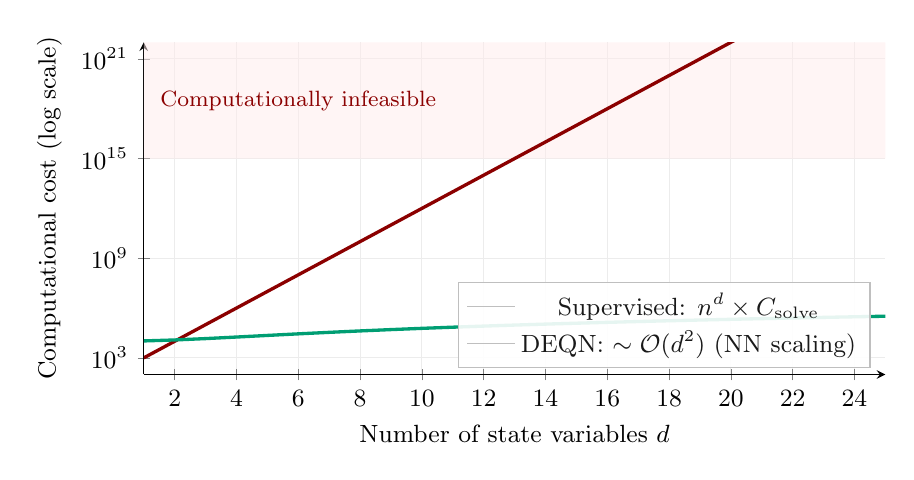
\begin{tikzpicture}
\begin{axis}[
    width=11cm, height=5.8cm,
    xlabel={Number of state variables $d$},
    ylabel={Computational cost (log scale)},
    xlabel style={font=\small},
    ylabel style={font=\small},
    tick label style={font=\small},
    ymode=log,
    xmin=1, xmax=25, ymin=1e2, ymax=1e22,
    grid=major, grid style={gray!15},
    legend style={font=\small, at={(0.98,0.02)}, anchor=south east,
                  fill=white, fill opacity=0.9, draw=gray!50},
    axis lines=left,
]
    % Shaded infeasible region (draw first so it's behind)
    \addplot[name path=top, draw=none, domain=1:25]{1e22};
    \addplot[name path=thresh, draw=none, domain=1:25]{1e15};
    \addplot[fill=red!8, fill opacity=0.5, forget plot] fill between[of=top and thresh];

    \node[font=\footnotesize, darkred] at (axis cs:6,3e18) {Computationally infeasible};

    % Grid-based supervised
    \addplot[very thick, darkred, domain=1:25, samples=25]
        {10^(x) * 100};
    \addlegendentry{Supervised: $n^d \times C_{\text{solve}}$}

    % DEQN
    \addplot[very thick, softgreen, domain=1:25, samples=25]
        {500 * x^2 + 1e4};
    \addlegendentry{DEQN: $\sim \mathcal{O}(d^2)$ (NN scaling)}
\end{axis}
\end{tikzpicture}
\end{center}

\vspace{-0.2cm}
{\small Supervised approaches hit the wall around $d \approx 5$--$8$.  DEQNs scale gracefully to $d > 100$.}
\end{frame}

% --- DEQN Key Recap ---
\begin{frame}{DEQN: Key Recap}
\begin{columns}[T]
\column{0.32\textwidth}
\begin{block}{Replace Labels}
\centering
\small
Instead of labeled data $(\x_i, y_i)$, use the economic equilibrium equations $G(\cdot) = 0$ as the loss.
\end{block}

\column{0.32\textwidth}
\begin{block}{Replace Grids}
\centering
\small
Instead of $n^d$ grid points, use a neural network $\mathcal{N}_\rho$ that maps states to policies \emphc{globally}.
\end{block}

\column{0.32\textwidth}
\begin{block}{Replace TI}
\centering
\small
Instead of time iteration with interpolation, use SGD on simulated paths from the model.
\end{block}
\end{columns}

\vspace{0.8em}
\begin{center}
\textbf{Result:} A method that scales to \emphc{hundreds of state variables} and runs on GPUs.
\end{center}
\end{frame}


% ============================================================================
% PART III: BROCK--MIRMAN BENCHMARK
% ============================================================================

\section{Brock--Mirman Benchmark}

% --- Brock-Mirman Setup ---
\begin{frame}{Brock--Mirman (1972): Setup}
\textbf{Social planner's problem:}
\[
\max_{\{C_t\}_{t=0}^{\infty}} \; \E{\sum_{t=0}^{\infty} \beta^t \ln(C_t)}
\]
subject to:
\[
K_{t+1} + C_t = z_t K_t^\alpha, \qquad \ln z_{t+1} = \varrho \ln z_t + \sigma_z \epsilon_{t+1}, \quad \epsilon_t \sim \mathcal{N}(0,1)
\]

\vspace{0.3em}
\textbf{Euler equation:}
\[
\frac{1}{C_t} = \beta \, \E{\frac{\alpha z_{t+1} K_{t+1}^{\alpha-1}}{C_{t+1}}}
\]

\vspace{0.3em}
\textbf{Analytical solution} (log utility, full depreciation $\delta = 1$):
\[
K_{t+1} = \beta \alpha \, K_t^\alpha, \qquad C_t = (1 - \beta\alpha) \, K_t^\alpha
\]
\end{frame}

% --- DEQN for Brock-Mirman ---
\begin{frame}{DEQN for Brock--Mirman}
\textbf{Step 1:} Parametrize the policy function with a neural network:
\[
C_t = \mathcal{N}_\rho(K_t, z_t) \qquad\text{(consumption as a function of state)}
\]

\vspace{0.3em}
\textbf{Step 2:} Define the equilibrium residual:
\[
G(K_t, z_t) = 1 - \beta \, \frac{C_t}{C_{t+1}} \cdot \alpha z_{t+1} K_{t+1}^{\alpha-1}
\]
where $K_{t+1} = z_t K_t^\alpha - \mathcal{N}_\rho(K_t, z_t)$ and $C_{t+1} = \mathcal{N}_\rho(K_{t+1}, z_{t+1})$.

\vspace{0.3em}
\textbf{Step 3:} Minimize the DEQN loss:
\[
\ell_\rho = \frac{1}{N}\sum_{i=1}^{N} \bigl|G(K_t^{(i)}, z_t^{(i)})\bigr|^2
\]

{\small We can \emphc{verify} the solution against the analytical benchmark.}
\end{frame}

% --- Notebook References ---
\begin{frame}{Hands-on Notebooks}
\textbf{Two notebooks} accompany this lecture:

\vspace{0.5em}
\begin{enumerate}
    \item \texttt{01\_Brock\_Mirman\_1972\_DEQN.ipynb}\\
    {\small Deterministic Brock--Mirman with analytical benchmark.}

    \vspace{0.3em}
    \item \texttt{02\_Brock\_Mirman\_Uncertainty\_DEQN.ipynb}\\
    {\small Stochastic version with TFP shocks ($\varrho > 0$, $\sigma_z > 0$).}
\end{enumerate}

\vspace{0.5em}
All notebooks are in the \texttt{code/} directory and on the course GitHub repository.

\vspace{0.5em}
{\small \textbf{Note:} Exercises (\texttt{03\_DEQN\_Exercises\_Blancs.ipynb}) build on these notebooks.}
\end{frame}

% --- HPC Quote ---
\begin{frame}{}
\vfill
\begin{center}
{\Large\itshape
``To pull a bigger wagon, it is easier to add more oxen\\
than to grow a gigantic ox.''}

\vspace{0.8cm}
{\normalsize --- Gropp, Lusk \& Skjellum (1999)}\\[4pt]
{\small\itshape Using MPI: Portable Parallel Programming}
\end{center}
\vfill
\end{frame}

% --- Data Parallelism ---
\begin{frame}{Data Parallelism for DEQNs}
\textbf{Idea:} distribute training data across \emphc{multiple workers} (GPUs/CPUs).

\vspace{0.4em}
\begin{center}
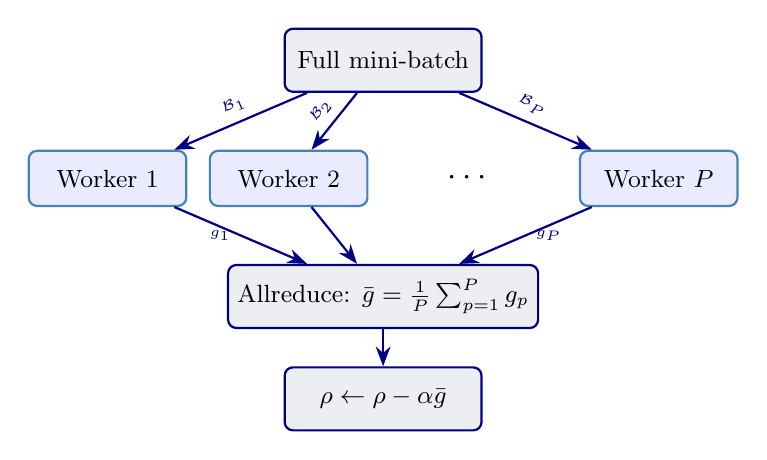
\begin{tikzpicture}[
    mlstep/.style={rectangle, draw=uzhblue, thick, fill=uzhgreylight,
        minimum width=2.5cm, minimum height=0.8cm, font=\small,
        rounded corners=3pt},
    worker/.style={rectangle, draw=softblue, thick, fill=blue!8,
        minimum width=2.0cm, minimum height=0.7cm, font=\small,
        rounded corners=3pt},
    arr/.style={-{Stealth[length=2.5mm]}, thick, uzhblue}
]
    \node[mlstep] (data) at (0,0) {Full mini-batch};
    \node[worker] (w1) at (-3.5,-1.5) {Worker 1};
    \node[worker] (w2) at (-1.2,-1.5) {Worker 2};
    \node[font=\large] (dots) at (1.1,-1.5) {$\cdots$};
    \node[worker] (wP) at (3.5,-1.5) {Worker $P$};

    \node[mlstep] (grad) at (0,-3.0) {Allreduce: $\bar{g} = \frac{1}{P}\sum_{p=1}^P g_p$};
    \node[mlstep] (upd) at (0,-4.3) {$\rho \leftarrow \rho - \alpha \bar{g}$};

    \draw[arr] (data) -- (w1) node[midway, above, font=\tiny, sloped] {$\mathcal{B}_1$};
    \draw[arr] (data) -- (w2) node[midway, above, font=\tiny, sloped] {$\mathcal{B}_2$};
    \draw[arr] (data) -- (wP) node[midway, above, font=\tiny, sloped] {$\mathcal{B}_P$};

    \draw[arr] (w1) -- (grad) node[midway, left, font=\tiny] {$g_1$};
    \draw[arr] (w2) -- (grad);
    \draw[arr] (wP) -- (grad) node[midway, right, font=\tiny] {$g_P$};

    \draw[arr] (grad) -- (upd);
\end{tikzpicture}
\end{center}

\vspace{0.2em}
{\small Implemented via \textbf{Horovod}/MPI. Each worker computes a local gradient; \emphc{allreduce} averages them.}
\end{frame}

% --- Scalability Results ---
\begin{frame}{Scalability Results}
\begin{center}
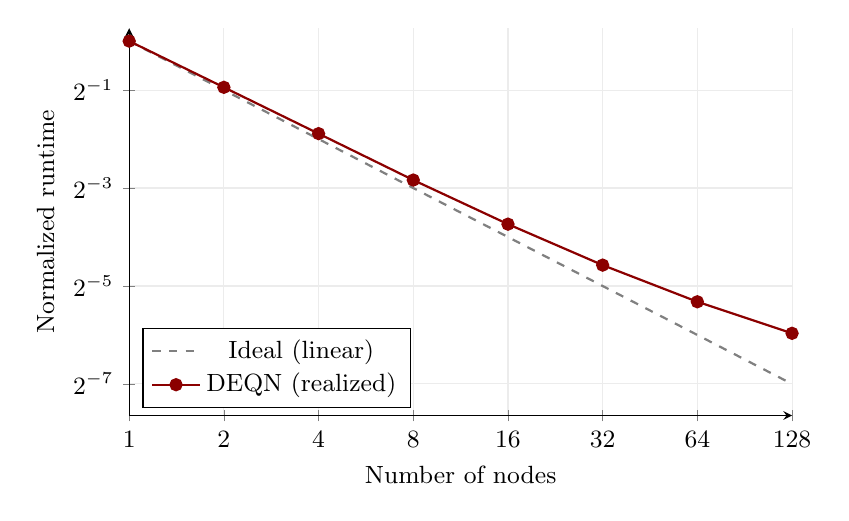
\begin{tikzpicture}
\begin{axis}[
    width=10cm, height=6.5cm,
    xlabel={Number of nodes},
    ylabel={Normalized runtime},
    xlabel style={font=\small},
    ylabel style={font=\small},
    tick label style={font=\small},
    xmode=log, ymode=log,
    log basis x=2, log basis y=2,
    xmin=1, xmax=128, ymin=0.005, ymax=1.2,
    grid=major, grid style={gray!15},
    legend style={font=\small, at={(0.02,0.02)}, anchor=south west},
    axis lines=left,
    xtick={1,2,4,8,16,32,64,128},
    xticklabels={1,2,4,8,16,32,64,128},
]
    % Ideal scaling
    \addplot[thick, dashed, gray, domain=1:128, samples=8]
        {1/x};
    \addlegendentry{Ideal (linear)}

    % Realized scaling (slightly worse)
    \addplot[thick, darkred, mark=*, mark size=2pt]
        coordinates {
            (1, 1.0) (2, 0.52) (4, 0.27) (8, 0.14)
            (16, 0.075) (32, 0.042) (64, 0.025) (128, 0.016)
        };
    \addlegendentry{DEQN (realized)}
\end{axis}
\end{tikzpicture}
\end{center}

{\small Near-linear scaling up to 128 nodes. Communication overhead is negligible for typical network sizes.}
\end{frame}


% ============================================================================
% PART IV: PRACTICAL TOOLS
% ============================================================================

\section{Practical Tools: NAS \& Loss Normalization}

% --- Why Architecture Matters ---
\begin{frame}{Why Architecture Matters}
\begin{columns}[T]
\column{0.52\textwidth}
\textbf{Same data, different architectures:}
\vspace{0.3cm}
\begin{itemize}
    \item 1 layer, 16 units $\;\Rightarrow\;$ MAE $= 0.08$
    \item 2 layers, 64 units $\;\Rightarrow\;$ MAE $= 0.01$
    \item 5 layers, 256 units $\;\Rightarrow\;$ MAE $= 0.003$
    \item 10 layers, 512 units $\;\Rightarrow\;$ MAE $= 0.02$ (overfit)
\end{itemize}
\vspace{0.3cm}
Architecture choice can matter \emphc{more than training duration}.

\column{0.45\textwidth}
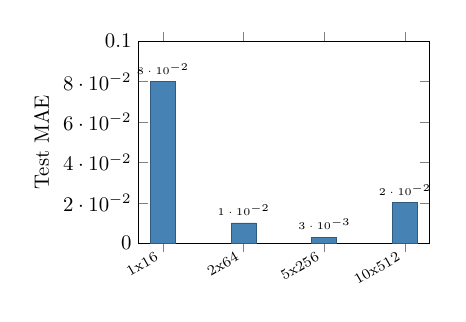
\begin{tikzpicture}[scale=0.75, transform shape]
    \begin{axis}[
        ybar,
        width=6.5cm, height=5cm,
        ylabel={Test MAE},
        symbolic x coords={1x16, 2x64, 5x256, 10x512},
        xtick=data,
        x tick label style={font=\scriptsize, rotate=30, anchor=east},
        ymin=0, ymax=0.1,
        bar width=12pt,
        nodes near coords,
        every node near coord/.append style={font=\tiny},
        nodes near coords align={vertical},
    ]
    \addplot[fill=softblue, draw=softblue!70!black] coordinates {
        (1x16, 0.08) (2x64, 0.01) (5x256, 0.003) (10x512, 0.02)
    };
    \end{axis}
\end{tikzpicture}
\end{columns}
\end{frame}

% --- NAS Method Comparison ---
\begin{frame}{Neural Architecture Search: Method Comparison}
\begin{center}
\renewcommand{\arraystretch}{1.3}
{\small
\begin{tabular}{@{}lcccc@{}}
\toprule
\textbf{Property} & \textbf{Grid} & \textbf{Random} & \textbf{Bayesian} & \textbf{Hyperband} \\
\midrule
Computational cost & $\mathcal{O}(k^d)$ & $\mathcal{O}(n)$ & $\mathcal{O}(n)$ & $\mathcal{O}(n \log n)$ \\
Sample efficiency & Low & Medium & \emphc{High} & High \\
Parallelisable & Fully & Fully & Limited & Partially \\
Handles interactions & No & Partially & \emphc{Yes} & No \\
Early stopping & No & No & No & \emphc{Yes} \\
Implementation & Trivial & Trivial & Moderate & Moderate \\
\bottomrule
\end{tabular}
}
\end{center}

\vspace{0.4cm}
\textbf{Practical advice:}
\begin{itemize}
    \item \textbf{Quick exploration:} Random search (strong baseline)
    \item \textbf{Limited budget:} Bayesian optimisation (sample-efficient)
    \item \textbf{Large search space:} Hyperband (aggressive early stopping)
\end{itemize}
\end{frame}

% --- Grid vs Random ---
\begin{frame}{Grid vs.\ Random --- Why Random Wins}
\begin{center}
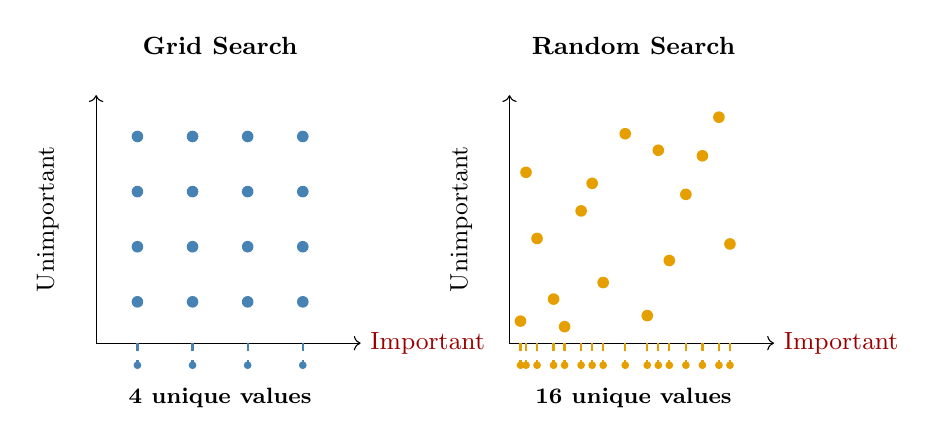
\begin{tikzpicture}[scale=0.7]
    % --- Left panel: Grid ---
    \begin{scope}[shift={(0,0)}]
        \node[font=\small\bfseries] at (2.25,5.4) {\textbf{Grid Search}};
        \draw[->] (0,0) -- (4.8,0) node[right,font=\small] {\emphc{Important}};
        \draw[->] (0,0) -- (0,4.5);
        \node[font=\small, rotate=90, anchor=south] at (-0.5,2.25) {Unimportant};
        \foreach \xi in {0.75,1.75,2.75,3.75} {
            \foreach \yi in {0.75,1.75,2.75,3.75} {
                \fill[softblue] (\xi,\yi) circle (3pt);
            }
        }
        \foreach \xi in {0.75,1.75,2.75,3.75} {
            \draw[softblue, thick, dashed] (\xi,0) -- (\xi,-0.4);
            \fill[softblue] (\xi,-0.4) circle (2pt);
        }
        \node[font=\footnotesize] at (2.25,-1.0) {\textbf{4 unique values}};
    \end{scope}

    % --- Right panel: Random ---
    \begin{scope}[shift={(7.5,0)}]
        \node[font=\small\bfseries] at (2.25,5.4) {\textbf{Random Search}};
        \draw[->] (0,0) -- (4.8,0) node[right,font=\small] {\emphc{Important}};
        \draw[->] (0,0) -- (0,4.5);
        \node[font=\small, rotate=90, anchor=south] at (-0.5,2.25) {Unimportant};
        \fill[softorange] (0.3,3.1) circle (3pt);
        \fill[softorange] (0.8,0.8) circle (3pt);
        \fill[softorange] (1.3,2.4) circle (3pt);
        \fill[softorange] (1.7,1.1) circle (3pt);
        \fill[softorange] (0.5,1.9) circle (3pt);
        \fill[softorange] (2.1,3.8) circle (3pt);
        \fill[softorange] (2.5,0.5) circle (3pt);
        \fill[softorange] (2.9,1.5) circle (3pt);
        \fill[softorange] (3.2,2.7) circle (3pt);
        \fill[softorange] (3.5,3.4) circle (3pt);
        \fill[softorange] (3.8,4.1) circle (3pt);
        \fill[softorange] (1.0,0.3) circle (3pt);
        \fill[softorange] (1.5,2.9) circle (3pt);
        \fill[softorange] (0.2,0.4) circle (3pt);
        \fill[softorange] (2.7,3.5) circle (3pt);
        \fill[softorange] (4.0,1.8) circle (3pt);
        \foreach \xi in {0.2,0.3,0.5,0.8,1.0,1.3,1.5,1.7,2.1,2.5,2.7,2.9,3.2,3.5,3.8,4.0} {
            \draw[softorange, thick, dashed] (\xi,0) -- (\xi,-0.4);
            \fill[softorange] (\xi,-0.4) circle (2pt);
        }
        \node[font=\footnotesize] at (2.25,-1.0) {\textbf{16 unique values}};
    \end{scope}
\end{tikzpicture}
\end{center}

\vspace{0.2cm}
When only one dimension matters, grid wastes $\frac{3}{4}$ of its budget
on the \emph{unimportant} axis. Random explores the important axis \emphc{4$\times$} more densely.
\end{frame}

% --- Bayesian Optimization ---
\begin{frame}{Bayesian Optimisation}
\begin{columns}[T]
\column{0.55\textwidth}
\textbf{Idea:} Build a \emph{surrogate model} of $f(\text{HP}) \to \text{loss}$ and use it to choose the next trial \emph{intelligently}.

\vspace{0.3cm}
\begin{enumerate}
    \item Fit a Gaussian process (GP) to observed trials
    \item Compute an \emphc{acquisition function} (e.g., Expected Improvement)
    \item Evaluate the HP with highest acquisition value
    \item Update the GP and repeat
\end{enumerate}

\vspace{0.3cm}
\textbf{Key advantage:} \emphc{Sample-efficient} --- exploits structure in the response surface.

\column{0.42\textwidth}
\begin{block}{Expected Improvement}
\vspace{-0.2cm}
\[
    \text{EI}(\x) = \E{\max(f^* - f(\x), 0)}
\]
\vspace{-0.2cm}
\begin{itemize}
    \item $f^*$: best observed value
    \item Balances \emph{exploration} (high uncertainty) and \emph{exploitation} (low predicted loss)
\end{itemize}
\end{block}
\end{columns}
\end{frame}

% --- Connection to Economics ---
\begin{frame}{NAS for Computational Economics}
\textbf{Where NAS matters in computational economics:}

\vspace{0.3cm}
\begin{enumerate}
    \item \textbf{Surrogate models:} Replace expensive simulations (e.g., climate IAMs) with NNs --- architecture determines approximation quality.

    \vspace{0.2cm}
    \item \textbf{DSGE policy functions:} Deep equilibrium nets use NNs to approximate policy/value functions. \emphc{Architecture search over the policy network} can improve convergence.

    \vspace{0.2cm}
    \item \textbf{High-dimensional problems:} As $d$ grows (many state variables), the architecture must scale. NAS automates this adaptation.

    \vspace{0.2cm}
    \item \textbf{Reproducibility:} Automated search documents \emph{which} architectures were tried, making results more transparent than ``we chose 3 layers with 64 units.''
\end{enumerate}
\end{frame}

% ---- Loss Normalization Section ----

% --- Motivation: Multi-Component Losses ---
\begin{frame}{Multi-Component Losses in DEQNs}
\textbf{Many problems require minimising \emph{several} loss terms simultaneously:}

\vspace{0.3cm}
\begin{columns}[T]
\column{0.50\textwidth}
\textbf{Deep equilibrium nets (DEQNs):}
\begin{itemize}
    \item Euler equation residuals
    \item Budget constraints
    \item Market clearing
\end{itemize}

\vspace{0.3cm}
\textbf{Physics-informed NNs (PINNs):}
\begin{itemize}
    \item PDE residual $\mathcal{L}_\text{PDE}$
    \item Boundary conditions $\mathcal{L}_\text{BC}$
    \item Initial conditions $\mathcal{L}_\text{IC}$
\end{itemize}

\column{0.47\textwidth}
\begin{alertblock}{Core challenge}
These loss components often live at \emphc{vastly different scales}.
\end{alertblock}

\vspace{0.3cm}
With equal weights:
\begin{itemize}
    \item Large-scale component dominates gradients
    \item Small-scale component is \emphc{ignored}
    \item The network effectively solves a \emph{single-task} problem
\end{itemize}
\end{columns}
\end{frame}

% --- The Scale Mismatch Problem ---
\begin{frame}{The Scale Mismatch Problem}
\textbf{Example:} IRBC model with $N=10$ countries has three types of residuals:

\vspace{0.3em}
\begin{center}
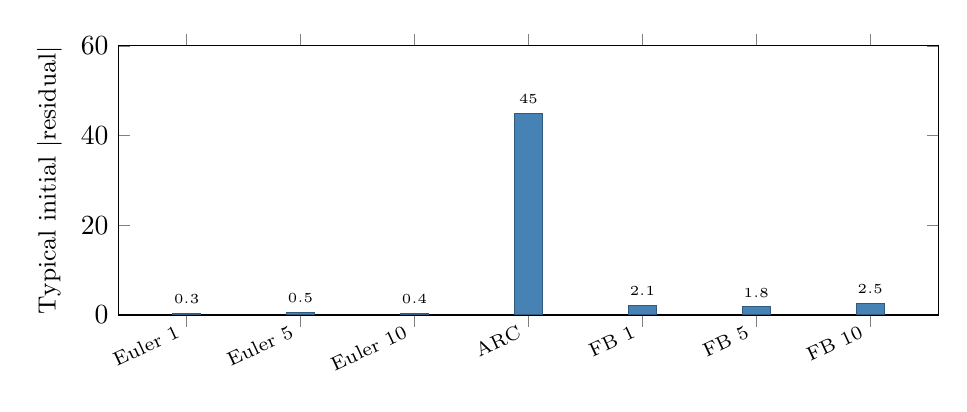
\begin{tikzpicture}
\begin{axis}[
    ybar,
    width=12cm, height=5cm,
    ylabel={Typical initial $|\text{residual}|$},
    ylabel style={font=\small},
    symbolic x coords={Euler 1, Euler 5, Euler 10, ARC, FB 1, FB 5, FB 10},
    xtick=data,
    x tick label style={font=\scriptsize, rotate=25, anchor=east},
    ymin=0, ymax=60,
    bar width=10pt,
    nodes near coords,
    every node near coord/.append style={font=\tiny},
    nodes near coords align={vertical},
    legend style={font=\scriptsize, at={(0.98,0.98)}, anchor=north east},
]
    \addplot[fill=softblue, draw=softblue!70!black] coordinates {
        (Euler 1, 0.3) (Euler 5, 0.5) (Euler 10, 0.4) (ARC, 45) (FB 1, 2.1) (FB 5, 1.8) (FB 10, 2.5)
    };
\end{axis}
\end{tikzpicture}
\end{center}

\vspace{0.2em}
\begin{itemize}
    \item The \emphc{aggregate resource constraint} (ARC) is $\sim\!100\times$ larger than the Euler residuals
    \item With equal weighting: $\nabla_\rho \ell \approx \nabla_\rho \ell_{\text{ARC}}$---the network \emphc{only} learns to clear markets
    \item Euler equations and complementarity conditions are \emphc{effectively ignored}
\end{itemize}
\end{frame}

% --- Gradient Dominance ---
\begin{frame}{Gradient Dominance: Why Na\"ive Weighting Fails}
\textbf{Total loss:} $\ell = \sum_{k=1}^K \ell_k$. The gradient is:
\[
\nabla_\rho \ell = \sum_{k=1}^K \nabla_\rho \ell_k
\]

\vspace{0.2em}
When $\ell_j \gg \ell_k$ for some $j$:
\begin{itemize}
    \item $\|\nabla_\rho \ell_j\| \gg \|\nabla_\rho \ell_k\|$~~$\Rightarrow$~~the update direction is dominated by component $j$
    \item Components $k \neq j$ may even \emphc{increase} during training
    \item The network converges to a solution that satisfies \emph{one} equation well but violates the others
\end{itemize}

\vspace{0.3em}
\begin{columns}[T]
\column{0.48\textwidth}
\begin{alertblock}{Na\"ive: $w_k = 1$ for all $k$}
\begin{itemize}
    \item Large-scale loss dominates
    \item Small losses stagnate or worsen
    \item Effectively single-task learning
\end{itemize}
\end{alertblock}

\column{0.48\textwidth}
\begin{exampleblock}{Adaptive: $w_k$ adjusted dynamically}
\begin{itemize}
    \item All loss components contribute equally to the gradient direction
    \item The network balances all equilibrium conditions
    \item True multi-task learning
\end{itemize}
\end{exampleblock}
\end{columns}
\end{frame}

% --- Alternative Approaches ---
\begin{frame}{Approaches to Loss Balancing}
\begin{center}
\renewcommand{\arraystretch}{1.3}
{\small
\begin{tabular}{@{}p{3cm}p{4.5cm}p{4.5cm}@{}}
\toprule
\textbf{Method} & \textbf{Idea} & \textbf{Limitation} \\
\midrule
Equal weights & $w_k = 1/K$ & Ignores scale differences entirely \\[2pt]
Manual tuning & Hand-pick $w_k$ & Tedious; does not adapt during training \\[2pt]
Inverse-loss & $w_k \propto 1/\ell_k$ & Oscillates: raises weight on noisy components \\[2pt]
GradNorm \newline (Chen et al., 2018) & Match gradient norms across tasks & Requires per-task gradient computation; expensive \\[2pt]
Uncertainty weighting \newline (Kendall et al., 2018) & Learn $\sigma_k$: $w_k \propto 1/(2\sigma_k^2)$ & Extra parameters; can collapse \\[2pt]
\emphc{ReLoBRaLo} \newline (Bischof et al., 2021) & Relative ratios + random lookback + smoothing & \emphc{Lightweight; robust; no extra params to learn} \\
\bottomrule
\end{tabular}
}
\end{center}

\vspace{0.3em}
{\small ReLoBRaLo's appeal: no gradient-norm computation, no extra learnable parameters, and strong empirical performance across domains (PINNs, DEQNs, multi-task regression).}
\end{frame}

% --- ReLoBRaLo ---
\begin{frame}{ReLoBRaLo --- Relative Loss Balancing with Random Lookback}
\begin{columns}[T]
\column{0.55\textwidth}
\textbf{Key innovations} (Bischof et al., 2021):

\vspace{0.2cm}
\begin{enumerate}
    \item \textbf{Relative balancing:} Use \emph{ratios} $\mathcal{L}_i^{(t)} / \mathcal{L}_i^{(t-1)}$ instead of absolute values

    \vspace{0.2cm}
    \item \textbf{Random lookback:} With probability $\rho$, compare to \emphc{initial losses} $\mathcal{L}_i^{(0)}$ instead of the previous step

    \vspace{0.2cm}
    \item \textbf{Exponential smoothing:} Blend new weights with history via $\alpha$
\end{enumerate}

\column{0.42\textwidth}
\begin{block}{Why random lookback?}
\begin{itemize}
    \item Prevents weight drift
    \item ``Resets'' to global perspective
    \item Stabilises training
    \item Like simulated annealing for weights
\end{itemize}
\end{block}
\end{columns}
\end{frame}

% --- ReLoBRaLo Algorithm ---
\begin{frame}{ReLoBRaLo --- Algorithm}
\begin{block}{Weight update at epoch $t$}
\begin{algorithmic}[1]
\STATE Compute losses $\mathcal{L}_1^{(t)}, \ldots, \mathcal{L}_K^{(t)}$
\STATE \textbf{Step-wise weights:}\; $\hat{w}_i^{(t)} = \operatorname{softmax}_i\!\Bigl(\frac{\mathcal{L}_i^{(t)}}{T \cdot \mathcal{L}_i^{(t-1)}}\Bigr) \cdot K$
\STATE \textbf{Baseline weights:}\; $\hat{w}_i^{(0)} = \operatorname{softmax}_i\!\Bigl(\frac{\mathcal{L}_i^{(t)}}{T \cdot \mathcal{L}_i^{(0)}}\Bigr) \cdot K$
\STATE \textbf{Combine with random lookback:}
\[
    w_i^{(t)} = \alpha \Bigl[\rho \, w_i^{(t-1)} + (1-\rho) \, \hat{w}_i^{(0)}\Bigr] + (1-\alpha) \, \hat{w}_i^{(t)}
\]
\end{algorithmic}
\end{block}

\vspace{0.3cm}
\begin{itemize}
    \item $\alpha$: smoothing --- how much to trust the historical weights
    \item $\rho$: lookback probability --- how often to reset to initial comparison
    \item $T$: temperature --- sharpness of the softmax
\end{itemize}
\end{frame}

% --- ReLoBRaLo Results ---
\begin{frame}{ReLoBRaLo --- Experiment Results}
\begin{center}
\renewcommand{\arraystretch}{1.3}
{\small
\begin{tabular}{@{}lccc@{}}
\toprule
 & \textbf{Equal weights} & \textbf{Inverse-loss} & \textbf{ReLoBRaLo} \\
\midrule
$f_A$ mean error & $5.2 \times 10^{-1}$ & $8.1 \times 10^{-2}$ & $\bm{3.4 \times 10^{-3}}$ \\
$f_B$ mean error & $3.7 \times 10^{0}$ & $1.5 \times 10^{0}$ & $\bm{8.2 \times 10^{-1}}$ \\
$f_C$ mean error & $\bm{4.5 \times 10^{1}}$ & $9.8 \times 10^{1}$ & $5.1 \times 10^{1}$ \\
\midrule
Total rel.\ error & 1.00 & 0.41 & \emphc{0.12} \\
\bottomrule
\end{tabular}
}
\end{center}

\vspace{0.3cm}
\begin{itemize}
    \item \textbf{Equal:} $f_C$ dominates training; $f_A$ is essentially \emphc{not learned}
    \item \textbf{Inverse-loss:} Improves $f_A$, but introduces oscillations
    \item \textbf{ReLoBRaLo:} All three functions well approximated; $\sim 8\times$ lower total error
\end{itemize}
\end{frame}

% --- Connection to DEQNs ---
\begin{frame}{Loss Balancing for DEQNs}
\begin{columns}[T]
\column{0.50\textwidth}
\textbf{DSGE / Deep equilibrium nets:}
\begin{itemize}
    \item Euler equations at different scales
    \item Budget constraint residuals
    \item Market clearing conditions
    \item Each may have different units and magnitudes
\end{itemize}

\vspace{0.3em}
$\Rightarrow$ ReLoBRaLo ensures all equilibrium conditions are learned, not just the largest.

\column{0.47\textwidth}
\textbf{ReLoBRaLo defaults:}
\begin{center}
\renewcommand{\arraystretch}{1.4}
\begin{tabular}{@{}clc@{}}
\toprule
\textbf{Symbol} & \textbf{Name} & \textbf{Default} \\
\midrule
$T$ & Temperature & $1.0$ \\
$\alpha$ & Smoothing & $0.999$ \\
$\rho$ & Lookback prob. & $0.999$ \\
\bottomrule
\end{tabular}
\end{center}

\vspace{0.3em}
\begin{block}{Practical guidance}
The defaults work well in most cases. Only $T$ needs occasional tuning.
\end{block}
\end{columns}
\end{frame}


% ============================================================================
% PART V: SCALING UP — THE IRBC MODEL
% ============================================================================

\section{Scaling Up --- The IRBC Model}

% --- Why International Models? ---
\begin{frame}{Why International Models?}
\begin{columns}[T]
\column{0.48\textwidth}
\textbf{Key questions in international macro:}
\begin{itemize}
    \item How do \emphc{capital flows} respond to productivity shocks?
    \item What governs \emphc{international risk sharing}?
    \item How do \emphc{trade imbalances} emerge?
\end{itemize}

\vspace{0.5em}
$\Rightarrow$ Need models with $N$ heterogeneous countries.

\vspace{0.3em}
$\Rightarrow$ State space: $2N$ dimensions (capital + TFP per country).

\column{0.48\textwidth}
\begin{center}
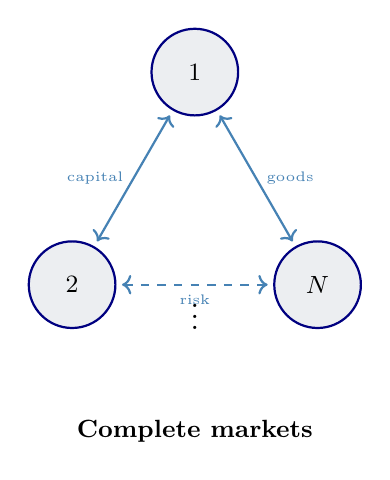
\begin{tikzpicture}[
    country/.style={circle, draw=uzhblue, thick, fill=uzhgreylight,
        minimum size=1.1cm, font=\small},
    flow/.style={<->, thick, softblue, shorten >=2pt, shorten <=2pt}
]
    \node[country] (c1) at (90:1.8) {$1$};
    \node[country] (c2) at (210:1.8) {$2$};
    \node[country] (c3) at (330:1.8) {$N$};
    \node[font=\large] at (270:1.2) {$\vdots$};

    \draw[flow] (c1) -- (c2) node[midway, left, font=\tiny] {capital};
    \draw[flow] (c1) -- (c3) node[midway, right, font=\tiny] {goods};
    \draw[flow, dashed] (c2) -- (c3) node[midway, below, font=\tiny] {risk};

    \node[below=0.3cm, font=\small\bfseries] at (0,-2.2) {Complete markets};
\end{tikzpicture}
\end{center}
\end{columns}
\end{frame}

% --- IRBC Model Overview ---
\begin{frame}{IRBC Model Overview}
\textbf{International Real Business Cycle (IRBC) model:}

\vspace{0.5em}
\begin{itemize}
    \item $N$ countries, each with \emphc{country-specific capital} $k^j$ and \emphc{TFP} $z^j$
    \item \emphc{Complete markets}: a social planner allocates resources with Pareto weights $\tau^j$
    \item \emphc{Irreversible investment}: $I^j \geq 0$ (cannot disinvest)
    \item \emphc{Capital adjustment costs}: $\Gamma^j = \frac{\kappa}{2} k^j \!\left(\frac{k^{j\prime}}{k^j} - 1\right)^{\!2}$
\end{itemize}

\vspace{0.5em}
\begin{block}{Dimensionality}
State: $\bm{s} = (k^1, \ldots, k^N, z^1, \ldots, z^N) \in \R^{2N}$\\
Policy: $(k^{1\prime}, \ldots, k^{N\prime}, \lambda, \mu^1, \ldots, \mu^N) \in \R^{2N+1}$
\end{block}
\end{frame}

% --- Preferences and Production ---
\begin{frame}{Preferences and Production}
\begin{columns}[T]
\column{0.48\textwidth}
\textbf{CRRA utility} for each country $j$:
\[
u^j(c) = \frac{c^{\,1 - 1/\gamma_j}}{1 - 1/\gamma_j}
\]

\begin{itemize}
    \item $\gamma_j$: intertemporal elasticity of substitution
    \item Heterogeneous: $\gamma_j \in [\gamma_{\min}, \gamma_{\max}]$
\end{itemize}

\vspace{0.3em}
\textbf{Social planner} maximizes:
\[
\max \; \sum_{t=0}^{\infty} \beta^t \, \E{\sum_{j=1}^{N} \tau^j \, u^j(c_t^j)}
\]

\column{0.48\textwidth}
\textbf{Production} in country $j$:
\[
Y^j = A_{\text{tfp}} \cdot \exp(z^j) \cdot (k^j)^\zeta
\]

\vspace{0.3em}
\textbf{TFP process} (AR(1)):
\[
z^{j\prime} = \rho_z \, z^j + \sigma_e \bigl(\varepsilon^j + \varepsilon^{\text{agg}}\bigr)
\]

\vspace{0.3em}
\begin{center}
{\small
\begin{tabular}{ll}
\toprule
$\beta = 0.99$ & $\zeta = 0.36$ \\
$\delta = 0.01$ & $\kappa = 0.50$ \\
$\rho_z = 0.95$ & $\sigma_e = 0.01$ \\
\bottomrule
\end{tabular}
}
\end{center}
\end{columns}
\end{frame}

% --- Equilibrium System ---
\begin{frame}{Equilibrium System}
\textbf{$2N+1$ equations in $2N+1$ unknowns:}

\vspace{0.3em}
\begin{itemize}
    \item \textbf{$N$ Euler equations} (relative error form):
    \[
    \frac{\beta\,\E{\lambda' \cdot \text{MPK}^{j\prime} - (1-\delta)\,\mu^{j\prime}} + \mu^j}{\lambda\,(1 + \Gamma_{k'})} - 1 = 0
    \]

    \item \textbf{Aggregate resource constraint} (1 equation):
    \[
    \sum_{j=1}^{N} \Bigl[Y^j + (1-\delta)\,k^j - k^{j\prime} - \Gamma^j - c^j\Bigr] = 0
    \]

    \item \textbf{$N$ Fischer--Burmeister conditions} (irreversibility):
    \[
    \text{FB}(\mu^j, I^j) = \mu^j + I^j - \sqrt{(\mu^j)^2 + (I^j)^2 + \varepsilon} = 0
    \]
\end{itemize}

\vspace{0.3em}
{\small Consumption is determined by $\lambda$: $c^j = (\lambda/\tau^j)^{-\gamma_j}$.}
\end{frame}

% --- DEQN for IRBC ---
\begin{frame}{DEQN Formulation for the IRBC}
\begin{center}
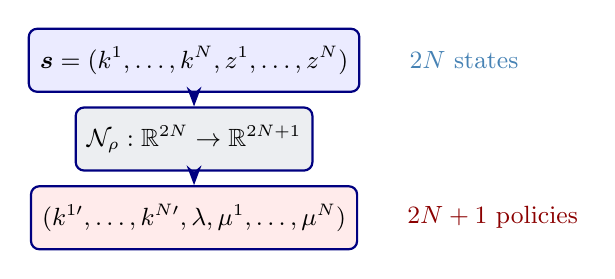
\begin{tikzpicture}[
    mlstep/.style={rectangle, draw=uzhblue, thick, fill=uzhgreylight,
        minimum width=3.0cm, minimum height=0.8cm, font=\small,
        rounded corners=3pt, inner sep=4pt},
    arr/.style={-{Stealth[length=2.5mm]}, thick, uzhblue}
]
    \node[mlstep, fill=blue!8] (state) at (0,0)
        {$\bm{s} = (k^1, \ldots, k^N, z^1, \ldots, z^N)$};
    \node[mlstep, fill=red!8] (policy) at (0,-2.0)
        {$(k^{1\prime}, \ldots, k^{N\prime}, \lambda, \mu^1, \ldots, \mu^N)$};
    \node[mlstep] (nn) at (0,-1.0)
        {$\mathcal{N}_\rho : \R^{2N} \to \R^{2N+1}$};

    \draw[arr] (state) -- (nn);
    \draw[arr] (nn) -- (policy);

    \node[right=0.5cm, font=\small, softblue] at (state.east) {$2N$ states};
    \node[right=0.5cm, font=\small, darkred] at (policy.east) {$2N+1$ policies};
\end{tikzpicture}
\end{center}

\vspace{0.3em}
\textbf{Loss:} sum of squared residuals over all equilibrium conditions:
\[
\ell_\rho = \frac{1}{B}\sum_{i=1}^{B} \left[\sum_{j=1}^{N} \bigl(\text{Euler}_j^{(i)}\bigr)^2 + \bigl(\text{ARC}^{(i)}\bigr)^2 + \sum_{j=1}^{N} \bigl(\text{FB}_j^{(i)}\bigr)^2\right]
\]

{\small Architecture: 2 $\times$ 64 hidden units, Swish activation, Softplus output (ensures positivity).}
\end{frame}

% --- Scalability in N ---
\begin{frame}{Scalability in $N$}
\begin{center}
\begin{tabular}{rrrrl}
\toprule
$N$ & \textbf{States} & \textbf{Policies} & \textbf{NN params} & \textbf{Grid pts ($n\!=\!10$)} \\
\midrule
2 & 4 & 5 & $\sim$4.7K & $10^4$ \\
4 & 8 & 9 & $\sim$5.3K & $10^8$ \\
10 & 20 & 21 & $\sim$6.7K & $10^{20}$ \\
50 & 100 & 101 & $\sim$17K & $10^{100}$ \\
100 & 200 & 201 & $\sim$30K & $10^{200}$ \\
\bottomrule
\end{tabular}
\end{center}

\vspace{0.5em}
\begin{itemize}
    \item NN parameters grow \emphc{linearly} in $N$ (only input/output layers scale)
    \item Grid methods grow \emphc{exponentially}: $10^{2N}$ points
    \item DEQN training cost per step: $\mathcal{O}(|\rho| \cdot B \cdot Q^{N+1})$
    \item For large $N$: replace tensor-product GH with monomial rules or QMC
\end{itemize}
\end{frame}

% --- From Brock-Mirman to IRBC ---
\begin{frame}{From Brock--Mirman to IRBC}
\begin{center}
\begin{tabular}{lll}
\toprule
& \textbf{Brock--Mirman} & \textbf{IRBC} \\
\midrule
Countries & 1 & $N$ \\
States & $(K, z)$ & $(k^1, \ldots, k^N, z^1, \ldots, z^N)$ \\
Policies & $C$ (or $s$) & $(k^{1\prime}, \ldots, k^{N\prime}, \lambda, \mu^1, \ldots, \mu^N)$ \\
Equations & 1 Euler & $N$ Euler $+$ 1 ARC $+$ $N$ FB \\
Constraints & none & irreversibility, adj.\ costs \\
Shocks & 1 & $N+1$ \\
Output act. & sigmoid & softplus \\
Analytical sol. & yes ($\delta=1$) & no \\
\bottomrule
\end{tabular}
\end{center}

\vspace{0.3em}
{\small The IRBC is a natural \emphc{scaling test} for the DEQN methodology.}
\end{frame}

% --- IRBC Notebook Reference ---
\begin{frame}{IRBC Notebook}
\textbf{Hands-on:} \texttt{04\_IRBC\_DEQN.ipynb}

\vspace{0.5em}
\begin{enumerate}
    \item Parameters \& steady state verification
    \item Gauss--Hermite quadrature setup
    \item Keras network definition
    \item Model equations (production, consumption, adjustment costs)
    \item Cost function with Euler, ARC, and FB residuals
    \item Two-phase training loop
    \item Convergence analysis \& policy function plots
    \item Economic diagnostics (consumption sharing, trade balance)
\end{enumerate}

\vspace{0.5em}
{\small Self-contained: all equations implemented inline, no external imports beyond TensorFlow/NumPy.}
\end{frame}


% ============================================================================
% PART VI: HANDS-ON EXERCISES
% ============================================================================

\section{Hands-on Exercises}

% --- Notebook Summary ---
\begin{frame}{Code Notebooks}
\begin{center}
\renewcommand{\arraystretch}{1.4}
{\small
\begin{tabular}{@{}lp{8cm}@{}}
\toprule
\textbf{Notebook} & \textbf{Description} \\
\midrule
\texttt{01\_Brock\_Mirman\_1972\_DEQN} & Deterministic Brock--Mirman model with analytical benchmark \\
\texttt{02\_Brock\_Mirman\_Uncertainty\_DEQN} & Stochastic Brock--Mirman with TFP shocks \\
\texttt{03\_DEQN\_Exercises\_Blancs} & Exercise problems (blanks to fill in) \\
\texttt{03\_DEQN\_Exercises\_Solutions} & Exercise solutions \\
\texttt{04\_IRBC\_DEQN} & Full IRBC model: multi-country DEQN with adjustment costs and irreversibility \\
\bottomrule
\end{tabular}
}
\end{center}

\vspace{0.5em}
All notebooks are in the \texttt{code/} directory. Requirements: \texttt{pip install -r requirements.txt}
\end{frame}

% --- Readings ---
\begin{frame}{Suggested Readings}
\begin{enumerate}
    \item \textbf{Azinovic, Gaegauf \& Scheidegger} (2022).\\
    {\small \emph{Deep Equilibrium Nets.} International Economic Review 63(4), 1471--1525.}

    \vspace{0.3em}
    \item \textbf{Fern\'{a}ndez-Villaverde, Nu\~{n}o \& Perla} (2024).\\
    {\small \emph{Taming the Curse of Dimensionality: Quantitative Economics with Deep Learning.} NBER Working Paper 33117.}

    \vspace{0.3em}
    \item \textbf{Chen, Didisheim \& Scheidegger} (2026).\\
    {\small \emph{Deep Surrogates for Finance: With an Application to Option Pricing.} Journal of Financial Economics 177, 104222.}

    \vspace{0.3em}
    \item \textbf{Friedl, K\"{u}bler, Scheidegger \& Usui} (2023).\\
    {\small \emph{Deep Uncertainty Quantification: With an Application to Integrated Assessment Models.} Working paper.}
\end{enumerate}

\vspace{0.5em}
All papers are in the \texttt{readings/} directory.
\end{frame}


% ============================================================================
% CLOSING
% ============================================================================

\begin{frame}{}
\begin{columns}[c]
\column{0.45\textwidth}
\begin{center}
{\Huge \textcolor{uzhblue}{\textbf{Questions?}}}

\vspace{0.8cm}
{\large Galo Nu\~{n}o}\\[2pt]
{\small Banco de Espa\~{n}a}\\[4pt]
{\large Simon Scheidegger}\\[2pt]
{\small HEC, University of Lausanne}\\[6pt]
{\scriptsize \url{https://www.galonuno.com/}}\\[2pt]
{\scriptsize \url{https://sites.google.com/site/simonscheidegger/}}

\vspace{0.6cm}
{\small Materials:~~\url{https://github.com/sischei/DEQN_Galo_03_2026}}
\end{center}

\column{0.45\textwidth}
\begin{center}
\textbf{Key references:}\\[6pt]
{\small
Azinovic, Gaegauf \& Scheidegger (2022)\\
\emph{Deep Equilibrium Nets}\\
International Economic Review
}
\end{center}
\end{columns}
\end{frame}

\end{document}
